\documentclass[11pt]{article}

\usepackage[margin=1in]{geometry}
\usepackage{amsmath}
\usepackage{amssymb}
\usepackage{booktabs}
\usepackage{graphicx}
\usepackage[hidelinks]{hyperref}
\usepackage[T1]{fontenc}
\usepackage[utf8]{inputenc}
\usepackage{lmodern}
\graphicspath{{../images/}}
\setlength{\emergencystretch}{3em}

\title{OpenMC-Informed Reactor Model\\[0.4em]
\large Physics, Numerics, and Web Application Coupling}
\author{}
\date{}

\begin{document}

\maketitle
\tableofcontents
\clearpage

\section{Purpose and model boundary}

This note is the physics and numerical-method reference for the \emph{current}
Reactor Kinetics Lab web application.  It follows the active modeling path from
the continuous-energy OpenMC reactor through published reference data, point
kinetics, the resolved four-group diffusion solver, and the Modelica
thermal-hydraulics coupling.

The notebooks are analysis and reference-data workspaces.  The Python backend
is the runtime source of truth and the React frontend presents its state.  The
retired homogeneous one-group model and its old Core and Transient Diffusion
backends are documented separately in
\texttt{legacy\_homogeneous\_reactor.pdf}; they are not frontend models.

\section{From the first diffusion model to OpenMC}

The project began with a homogeneous buckling estimate followed by a
one-group, two-dimensional annular diffusion model.  That work was useful for
learning leakage, critical-size searches, rod-worth scans, and sparse
eigenvalue methods.  It also exposed the weakness of selecting
engineering-effective one-group constants by hand: spectral effects, resolved
fuel geometry, and control-rod behavior could not be defended independently.

The next modeling stage therefore used continuous-energy Monte Carlo in
OpenMC.  An FRM-II-inspired involute natural-uranium concept was explored
first.  A concentric annular arrangement was then selected because it preserves
the main fuel/moderator heterogeneity while remaining practical for resolved
cell-wise MGXS generation and an axisymmetric diffusion model.  The design is
inspired by research-reactor layouts; it is not a replica of a licensed
facility.

\begin{figure}[ht]
  \centering
  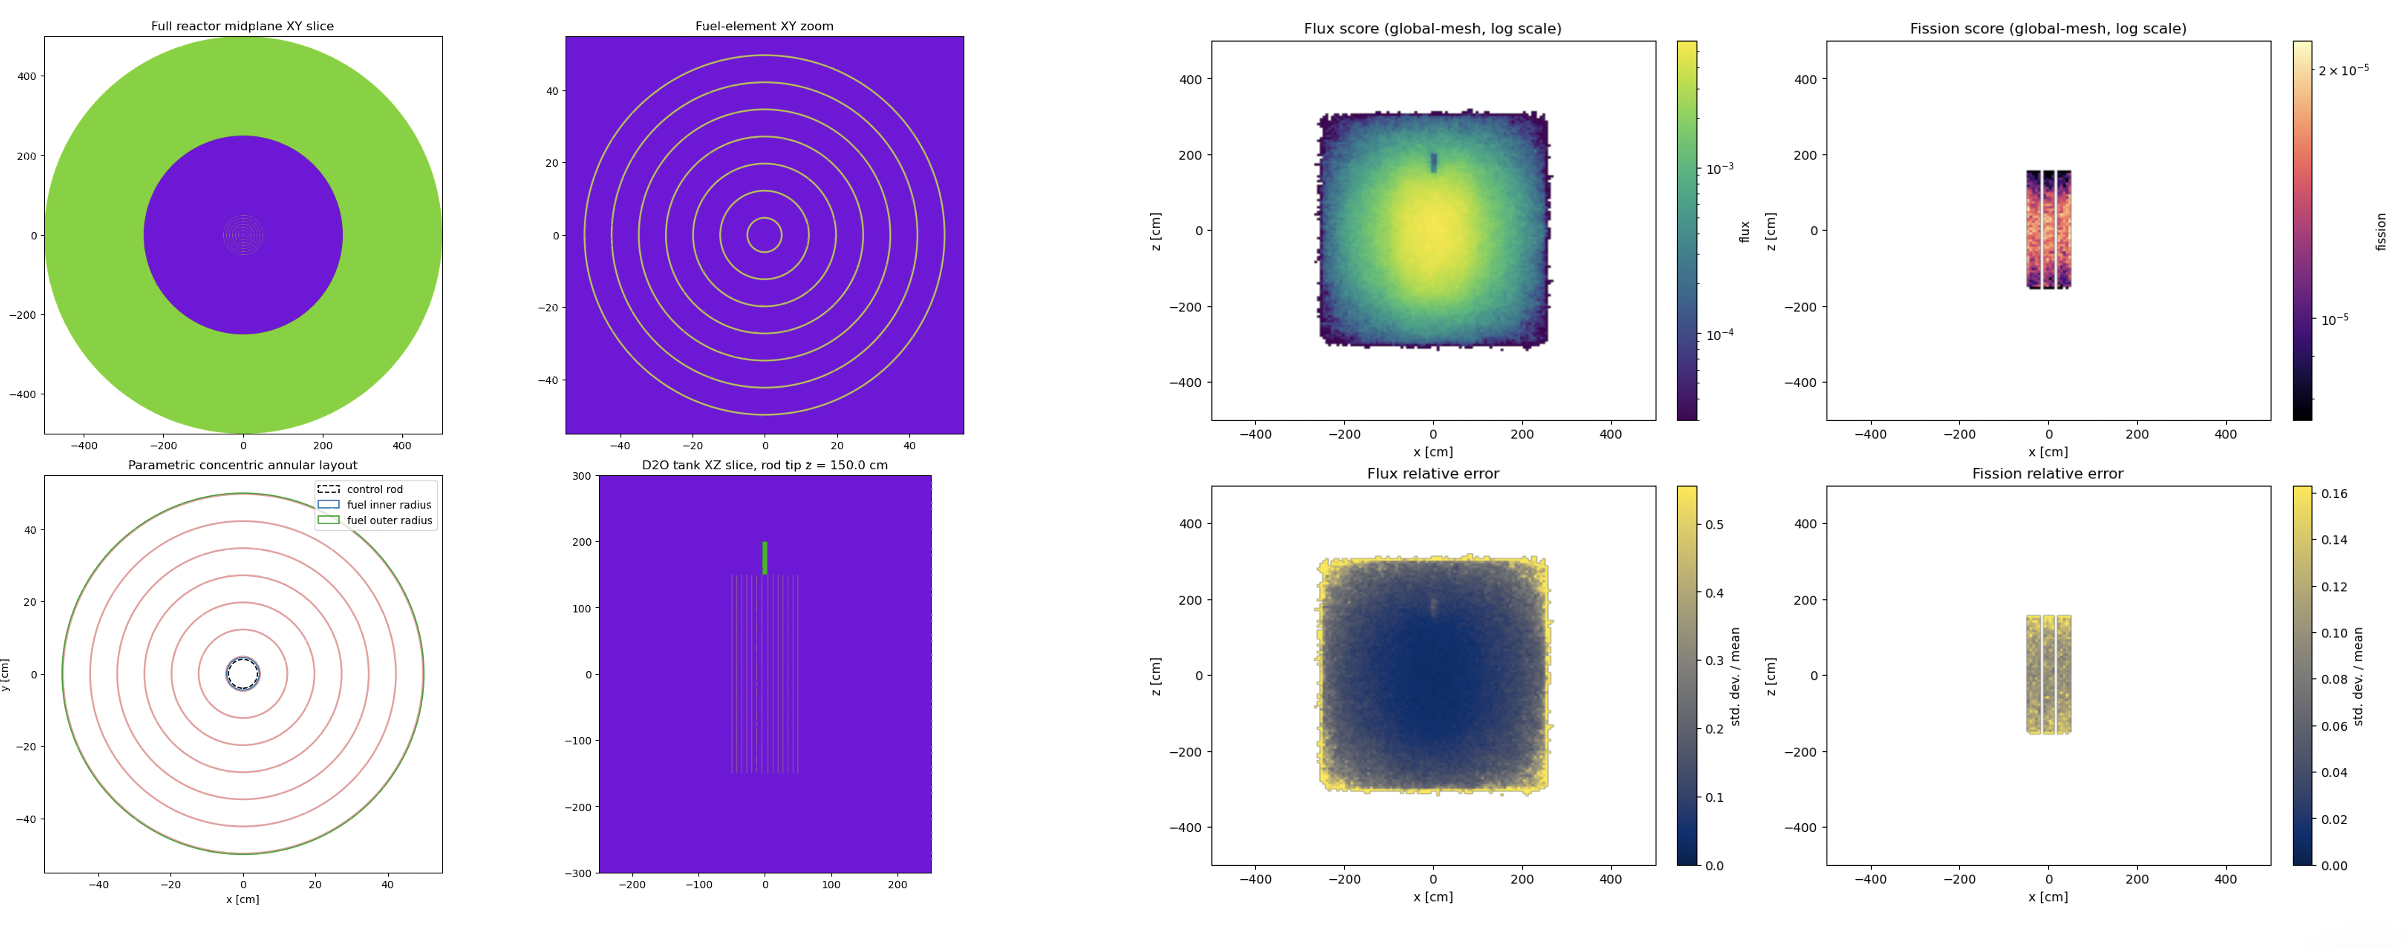
\includegraphics[width=0.96\textwidth]{coreModel.png}
  \caption{Development from exploratory reactor geometry to the resolved
  concentric OpenMC model.}
\end{figure}

\section{Current OpenMC reactor and published reference data}

The runtime neutronics reference is the tracked four-group publication under
\path{openmc/reference_data/concentric/group_sweep/group_4}.  Its
\texttt{model.xml} preserves seven fuel-ring cells, moderator and coolant
regions, a parked control-rod cell, and the surrounding D$_2$O and H$_2$O
regions.  The active fuel height is 300 cm and the fuel-element radius is
50 cm; the published diffusion geometry extends to a 250 cm moderator radius
and a 500 cm reflector radius.  These dimensions come from the publication,
not from the legacy one-group calibration.

OpenMC is run offline.  Normal web requests consume compact, versioned
artifacts rather than launching a Monte Carlo calculation:

\begin{center}
\small
\begin{tabular}{p{4.0cm}p{4.0cm}p{5.0cm}}
\toprule
Artifact & Runtime loader & Use \\
\midrule
\path{mgxs_constants.json} &
\path{kinetics_reference.py} and the MGXS adapter &
Delayed-neutron constants, generation time, resolved multigroup cross
sections, CE flux tallies, and the clean CE power mesh \\
\texttt{model.xml} &
\texttt{openmc\_mgxs\_adapter.py} &
Resolved cell names and radial/axial material boundaries \\
\texttt{rod\_worth.csv} &
\texttt{rod\_worth.py} &
Continuous-energy rod worth used by point kinetics \\
\path{reactivity_coefficients.csv} &
the reactivity-coefficient loader &
Fuel-temperature, moderator-temperature, and moderator-density feedback slopes \\
\bottomrule
\end{tabular}
\end{center}

Two clean-core references must not be conflated.  The independent
continuous-energy rod scan starts at $k_{\mathrm{eff}}=1.00224587$, or
$+224.084$ pcm, and defines the point-kinetics rod-worth curve.  The
continuous-energy run associated with the published four-group MGXS has
$k_{\mathrm{eff}}=1.00142016\pm21.75$ pcm and is the comparison reference for
the Core-page diffusion calculation.

\section{Overview page: point-kinetics transient model}

\subsection{Governing equations}

The Overview page uses the standard six-group delayed-neutron point-kinetics
system:
\begin{align}
\frac{dn}{dt} &= \frac{\rho - \beta}{\Lambda} n + \sum_{i=1}^{6}\lambda_i C_i,
\\
\frac{dC_i}{dt} &= \frac{\beta_i}{\Lambda} n - \lambda_i C_i,
\qquad i=1,\dots,6.
\end{align}

Here:
\begin{itemize}
  \item $n(t)$ is the normalized neutron population,
  \item $\rho$ is reactivity in $\Delta k/k$,
  \item $\beta = \sum_i \beta_i$ is the effective delayed-neutron fraction,
  \item $\Lambda$ is the prompt neutron generation time,
  \item $C_i$ is precursor concentration for delayed group $i$,
  \item $\lambda_i$ is the delayed-group decay constant.
\end{itemize}

\subsection{Constants used by the web app}

The current production constants in \texttt{config.py} are loaded from the
published four-group OpenMC MGXS export
\path{openmc/reference_data/concentric/group_sweep/group_4/outputs/mgxs_constants.json}.
The backend averages the fuel-ring delayed-neutron data with a fission-source
weight,
\[
w_j = \sum_g \left(\nu\Sigma_f\right)_{j,g}\Phi_{j,g},
\]
where $j$ indexes the resolved fuel-ring domains.  The fuel-ring $\beta_i$
values are \emph{averaged}, not summed across rings.  The prompt neutron
generation time is taken from the export's \texttt{prompt\_generation\_time\_s}
tally.

The resulting constants are:
\begin{align*}
\beta_{\mathrm{eff}} &= 0.00678910882978 = 678.91\ \mathrm{pcm}, \\
\Lambda &= 0.00417212833712\ \mathrm{s}.
\end{align*}

The six delayed groups are:

\begin{center}
\begin{tabular}{ccc}
\toprule
Group & $\beta_i$ & $\lambda_i$ [s$^{-1}$] \\
\midrule
1 & 0.000227917094163 & 0.0133443203744 \\
2 & 0.00119534670498 & 0.0326776283533 \\
3 & 0.00115198689522 & 0.120914791504 \\
4 & 0.00262514724228 & 0.304202879275 \\
5 & 0.00112075519129 & 0.855415421400 \\
6 & 0.000467955701846 & 2.87295916880 \\
\bottomrule
\end{tabular}
\end{center}

Displayed output is scaled from the nominal operating point
\[
P_0 = 20\ \mathrm{MW_{th}}, \qquad
\Phi_0 = 1.5\times 10^{12}\ \mathrm{n\,cm^{-2}\,s^{-1}},
\]
using
\[
P(t) = P_0 n(t), \qquad \Phi(t) = \Phi_0 n(t).
\]

The 20 MW value is the design point shared with the Modelica model.  The
absolute flux scale is different: it is still the peak-flux normalization
inherited from the retired one-group Estimate 2 calculation.  It is not
derived from the current OpenMC model and should be replaced by an
OpenMC-consistent absolute normalization in future work.  This legacy scale
changes the displayed value of total flux, but not the normalized point-
kinetics solution.

\subsection{Initial conditions}

On construction and reset, the backend initializes
\[
n(0)=1,\qquad
C_i(0)=\frac{\beta_i}{\Lambda\lambda_i}n(0).
\]
The rod starts at the interpolated continuous-energy critical insertion,
$x_{\mathrm{crit}}=26.5323\%$, time starts at zero, and the displayed power is
therefore 20 MW.  The thermal adapter is reset at that power.  If a compatible
FMU starts successfully, its initial effective fuel temperature, moderator
temperature, and moderator density are captured as the zero-feedback
reference.  This makes the coupled reset state internally critical even when
the FMU initial state differs from the temperatures used to generate the
OpenMC coefficient slopes.

\subsection{How rod motion enters the point model}

The point-kinetics solver does not compute rod worth from first principles during
runtime.  Instead it loads the OpenMC continuous-energy rod-worth table
\path{openmc/reference_data/concentric/rod_scan/results/rod_worth.csv}.
Reactivity is computed as
\[
\rho_{\mathrm{tot,pcm}}(x)
= \rho_{\mathrm{clean,pcm}} + \Delta \rho_{\mathrm{rod,pcm}}(x)
+ \rho_{\mathrm{scram,pcm}} + \rho_{\mathrm{fb,pcm}},
\]
where $x \in [0,1]$ is rod insertion fraction.  In the current calibration:
\begin{align*}
k_{\mathrm{clean}} &= 1.00224587, \\
\rho_{\mathrm{clean}} &= +224.084\ \mathrm{pcm}, \\
x_{\mathrm{crit}} &= 0.265323, \\
\Delta \rho_{\mathrm{rod}}(1.0) &= -1350.73\ \mathrm{pcm}, \\
\rho_{\mathrm{scram}} &= -450\ \mathrm{pcm}\ \text{when latched.}
\end{align*}

The backend interpolates linearly between the insertion points stored in the
CSV.  The older diffusion-derived rod-worth curve is not used here.  Legacy
calibration data remain only in the retired one-group backends and in the
nominal flux and geometry metadata described above.

\subsection{Thermal reactivity feedback}

The point model also adds thermal feedback when the Modelica FMU reports all
three effective feedback signals:
\texttt{T\_fuelEff}, \texttt{T\_moderatorEff}, and \texttt{rho\_m\_eff}.  The
coefficients are loaded from
\path{openmc/reference_data/concentric/reactivity_coefficients/results/reactivity_coefficients.csv}:
\begin{align*}
\alpha_f &= -2.138272335\ \mathrm{pcm/K}, \\
\alpha_{m,T} &= -10.72767894\ \mathrm{pcm/K}, \\
\alpha_{m,\rho} &= 20993.04779\ \mathrm{pcm/(g/cm^3)}.
\end{align*}

At reset, the current FMU effective state is stored as the zero-feedback
reference.  Runtime feedback is then
\[
\rho_{\mathrm{fb,pcm}} =
\alpha_f \left(T_{f,eff}-T_{f,0}\right)
+ \alpha_{m,T}\left(T_{m,eff}-T_{m,0}\right)
+ \alpha_{m,\rho}\left(\rho_{m,eff}-\rho_{m,0}\right).
\]
This preserves the existing critical startup behavior while still using the
OpenMC finite-difference slopes.  Thermal feedback is \textbf{FMI-only}: if the
FMU is unavailable and the fallback thermal model is active, the feedback terms
are reported as zero and are not added to reactivity.

\begin{figure}[ht]
  \centering
  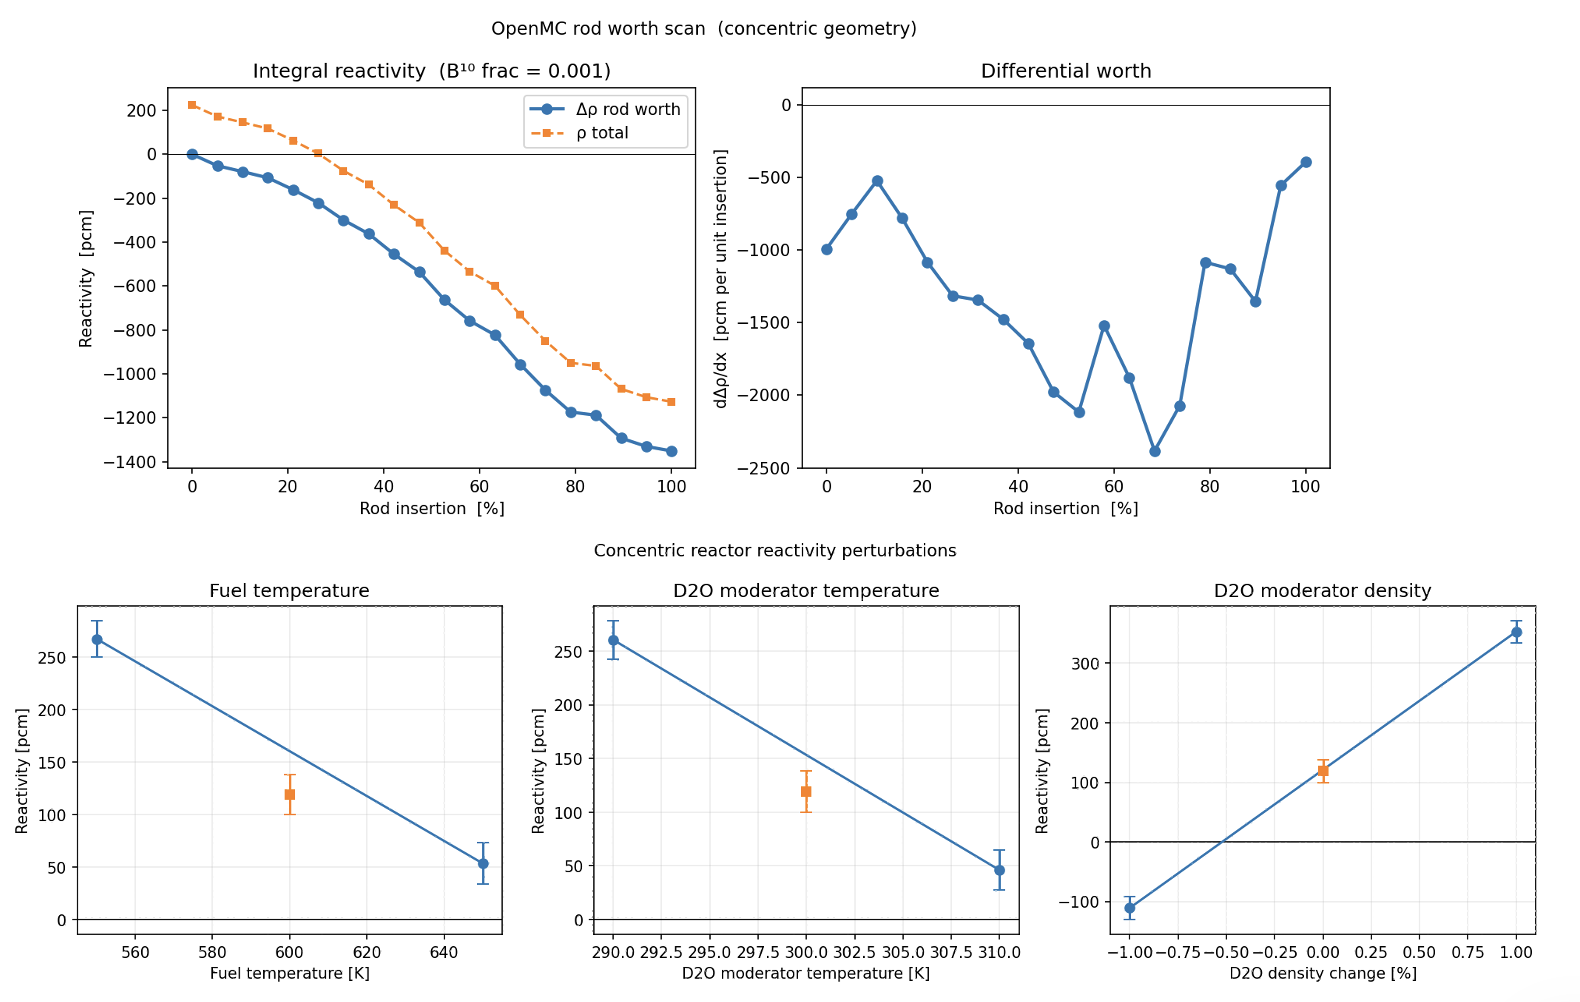
\includegraphics[width=0.78\textwidth]{reactivity.png}
  \caption{OpenMC perturbations provide the rod-worth and thermal-feedback
  terms used by point kinetics.}
\end{figure}

\subsection{Numerical method}

The point-kinetics equations are stiff, so the backend does not use explicit
Euler.  Instead \texttt{engine.py} advances both the neutron population and the
precursors implicitly at the new time level and then algebraically eliminates
the precursor unknowns.

Start from the backward-Euler discretization
\begin{align}
\frac{n^{k+1} - n^k}{\Delta t}
&=
\frac{\rho-\beta}{\Lambda} n^{k+1}
+ \sum_{i=1}^6 \lambda_i C_i^{k+1},
\\
\frac{C_i^{k+1} - C_i^k}{\Delta t}
&=
\frac{\beta_i}{\Lambda} n^{k+1} - \lambda_i C_i^{k+1}.
\end{align}

Solving the precursor equation for the new precursor gives
\[
C_i^{k+1}
=
\frac{C_i^k + \Delta t\,(\beta_i/\Lambda)\,n^{k+1}}
{1 + \lambda_i \Delta t},
\]
which is the relation already visible in the source.

Substituting that expression into the neutron balance yields
\[
\frac{n^{k+1} - n^k}{\Delta t}
=
\frac{\rho-\beta}{\Lambda} n^{k+1}
+ \sum_i \lambda_i
\frac{C_i^k + \Delta t\,(\beta_i/\Lambda)\,n^{k+1}}
{1+\lambda_i\Delta t}.
\]

Now separate the terms involving only known old-state data from the terms that
still multiply $n^{k+1}$:
\[
\frac{n^{k+1} - n^k}{\Delta t}
=
\sum_i \frac{\lambda_i C_i^k}{1+\lambda_i\Delta t}
+
\left[
\frac{\rho-\beta}{\Lambda}
+ \sum_i \frac{\lambda_i \Delta t\,\beta_i/\Lambda}{1+\lambda_i\Delta t}
\right] n^{k+1}.
\]

Rearranging gives one scalar solve for the new neutron population,
\[
n^{k+1}
=
\frac{n^k + \Delta t\sum_i \dfrac{\lambda_i C_i^k}{1+\lambda_i\Delta t}}
{1 - \Delta t\,\dfrac{\rho-\beta}{\Lambda}
 - \Delta t\sum_i
   \dfrac{\lambda_i \Delta t\,\beta_i/\Lambda}{1+\lambda_i\Delta t}}.
\]

In the implementation this matches the code variables
\texttt{delayed\_source}, \texttt{delayed\_coupling}, \texttt{numerator}, and
\texttt{denominator} in \texttt{engine.py}.  The precursor update then uses the
newly computed $n^{k+1}$.

Numerically, this matters because the prompt part of the kinetics is very fast
relative to the slowest delayed groups.  A naive explicit step would require a
much smaller $\Delta t$ for stability, while the semi-implicit update remains
well behaved for the chosen browser-friendly step size.

\subsection{How the Overview transient is operationalized}

The point-kinetics equations are not advanced continuously in a background
thread.  Instead \texttt{service.py} advances them \emph{opportunistically}
whenever the frontend polls or sends a command:
\begin{enumerate}
  \item compute elapsed wall time since the last request,
  \item cap that wall-time gap to avoid large jumps after browser pauses,
  \item multiply by the configured time-scale factor,
  \item then march the engine forward in repeated $0.02$ s internal steps.
\end{enumerate}

This architecture is a numerical simplification as much as a software one: the
browser sees a continuous transient, but the backend actually performs a sequence
of bounded substeps and samples history only every $0.25$ s.

The current runtime tuning in \texttt{config.py} is:
\begin{center}
\begin{tabular}{lc}
\toprule
Parameter & Value \\
\midrule
Integrator step & $0.02$ s \\
Thermal update batch & $0.10$ s \\
Maximum accepted wall-time gap & $0.20$ s \\
History sampling & $0.25$ s \\
History limit & $1200$ points \\
Time scale & $8\times$ wall clock \\
Frontend poll interval & $100$ ms \\
Automatic SCRAM threshold & $1000$ MW$_{\mathrm{th}}$ \\
\bottomrule
\end{tabular}
\end{center}


\section{Resolved multigroup diffusion for the Core page}

The frontend Core page uses a \textbf{resolved multigroup diffusion} chain that
derives its nuclear data from the OpenMC continuous-energy calculation.  This
is the only spatial neutronics visualization exposed in the frontend.

\subsection{Overview of the pipeline}

The multigroup workflow has five stages, all implemented as reusable Python
modules rather than notebook-only logic:

\begin{enumerate}
  \item \textbf{MGXS export} (\path{openmc/mgxs_export.py}):
        attach multigroup cross-section tallies to each resolved OpenMC cell
        (fuel rings, central channel, coolant, moderator, reflector, control
        rod), run an eigenvalue calculation, and write group constants plus
        delayed-neutron data as JSON and CSV.
  \item \textbf{Adapter and region mapping}
        (\path{backend/reactor_backend/openmc_mgxs_adapter.py}):
        parse the OpenMC \texttt{model.xml} to extract cell boundaries
        (z-cylinders and z-planes), load the canonical
        \texttt{mgxs\_constants.json}, validate the scattering contract,
        preserve the centimeter-based OpenMC units, and map each OpenMC cell to a
        \texttt{MultiGroupRegion} inside a \texttt{CylindricalLayeredModel2D}.
  \item \textbf{Finite-volume multigroup diffusion solver}
        (\path{backend/reactor_backend/multigroup_diffusion.py}):
        assemble per-group sparse spatial operators, solve the multigroup
        eigenvalue problem, and optionally scan rod insertion.
  \item \textbf{CE-referenced SPH research}
        (\path{backend/reactor_backend/multigroup_sph.py}):
        normalize the OpenMC and diffusion region-integrated fluxes to equal
        fission production, fit one factor per resolved region and energy
        group, apply the factors consistently to transport and reaction terms,
        and evaluate eigenvalue, flux, and power-shape acceptance criteria.
        This offline workflow is currently paused and its factors are not
        applied by the Core service.
  \item \textbf{Persistent preparation cache}
        (\path{backend/reactor_backend/multigroup_diffusion_cache.py}):
        fingerprint the MGXS data, mesh settings, optional offline SPH
        artifact, and solver configuration; build CSR matrices and a
        clean-core solution once, then persist them for fast reload.
\end{enumerate}

The command-line entry point is
\path{backend/openmc_to_diffusion.py}.  The notebook
\path{openmc/diffusion_concentric_reactor.ipynb} remains the analysis
interface, while the web application exposes a four-group rod-aware page
backed by the same adapter, clean-state persistent solution, and in-process
rodded solves.

\subsection{MGXS export from OpenMC}

The export module (\texttt{mgxs\_export.py}) takes a previously built OpenMC
\texttt{model.xml} and attaches multigroup tally objects to every resolved
cell domain.  The domain definitions are configurable; the resolved mode maps
each \texttt{fuel\_ring\_N} cell to its own domain label, plus the central
moderator channel, heavy-water coolant, outer moderator, reflector, and
parked control rod.  A frozen \texttt{MGXSExportConfig} dataclass captures the
particle count, batch schedule, energy-group edges (any CASMO structure from
1 to 70 groups), Legendre scattering order (P0, P1, P3, or P5), and the
delayed-neutron group count.

Two scattering representations are tallied from the same continuous-energy
run:
\begin{itemize}
  \item The \textbf{canonical diffusion export} uses non-$\nu$, uncorrected
        scattering (\texttt{scatter\_correction = null}).  The adapter prefers
        the \texttt{consistent scatter matrix} and falls back to
        \texttt{scatter matrix}.  Only the zeroth Legendre moment is passed to
        diffusion; higher moments are recorded and discarded.
  \item A \textbf{supplemental P0-corrected consistent scattering library}
        is tallied for OpenMC's own multigroup transport validation run.
        This correction is validation-only and is not written into the
        canonical diffusion JSON.
\end{itemize}

When \texttt{validation\_scatter\_correction = P0}, the export contract requires
\texttt{legendre\_order = 0}, because OpenMC does not apply that correction to
a higher-order Legendre library.  A higher-order canonical export can still be
read by the adapter, but the validation correction must be disabled for that
run and the diffusion path will retain only moment zero.

The diffusion coefficient is taken directly from OpenMC's transport
cross-section tally:
\[
D_g = \frac{1}{3\,\Sigma_{\mathrm{tr},g}} .
\]

This distinction is important.  OpenMC's P0 scatter correction modifies the
isotropic scattering data used by its multigroup \emph{transport} calculation
to represent part of the first angular moment.  The diffusion calculation
instead represents anisotropic migration through $\Sigma_{\mathrm{tr},g}$ in
$D_g$.  Its scattering source therefore uses the uncorrected non-$\nu$ P0
reaction-rate matrix.  The two calculations use different angular closures;
agreement of the OpenMC multigroup validation does not imply that the
diffusion approximation has been calibrated.

All neutronics quantities remain in OpenMC's native centimeter-based units:
$D$ in cm, macroscopic cross sections in cm$^{-1}$, and geometry and mesh
dimensions in cm.  No SI conversion is performed in the adapter.  This gives
$D\nabla^2\phi$ and $\Sigma\phi$ consistent units throughout the steady
solver.

Each export run produces:
\begin{itemize}
  \item \texttt{mgxs\_constants.json} --- nested group constants, delayed-neutron
        data, metadata for every domain, raw region/group CE flux tally means
        and standard deviations, and a cylindrical CE
        \texttt{kappa-fission} power-mesh tally;
  \item \texttt{group\_constants.csv} --- flat table of all group-constant rows;
  \item \texttt{delayed\_neutrons.csv} --- flat table of all delayed-neutron rows.
\end{itemize}

The raw CE flux tally is retained in fast-to-thermal group order without the
independent groupwise normalization used by the GeN-Foam auxiliary export.
This distinction is necessary because SPH requires relative region/group
reaction rates from one common Monte Carlo normalization.  The cylindrical
power tally supplies independent normalized radial and axial shape checks.

The notebook \texttt{openmc/exportMGXS.ipynb} runs group-count and
Legendre-order sweeps, storing each result under
\texttt{group\_sweep/group\_<N>/}.  It also runs an OpenMC multigroup
validation step that rebuilds an \texttt{mgxs.h5} library and solves the same
geometry in multigroup transport mode, producing the $\Delta\rho$ (MG $-$ CE)
values reported in the workflow document.

\subsection{Adapter: from OpenMC cells to diffusion regions}

The adapter (\texttt{openmc\_mgxs\_adapter.py}) is the bridge between the
OpenMC export and the diffusion solver.  It performs five operations:

\begin{enumerate}
  \item \textbf{Geometry extraction.}  Parses the OpenMC \texttt{model.xml}
        with Python's \texttt{ElementTree}, identifies every named cell, and
        extracts its radial and axial bounds from the z-cylinder and z-plane
        surfaces referenced in the cell's region specification.
  \item \textbf{Contract validation.}  Requires
        \texttt{scatter\_correction = null} in the export config so the P0
        scattering diagonal is not transport-corrected.  Rejects exports that
        are missing required domains (fuel rings, central channel, moderator,
        reflector) or whose MGXS domain labels do not match the XML cell names.
  \item \textbf{Scattering-matrix selection.}  Prefers
        \texttt{consistent scatter matrix}; falls back to \texttt{scatter matrix}.
        Discards any Legendre moments above P0 and interprets the stored matrix
        as $\Sigma_{s,g'\rightarrow g}$, with the first group index denoting the
        source group and the second the destination group.
  \item \textbf{Diffusion-coefficient validation.}  For every active
        region/group pair, checks that the exported coefficient is finite,
        positive, and consistent with
        $D_g=1/(3\Sigma_{\mathrm{tr},g})$ to numerical precision.
  \item \textbf{Inactive-group sanitization.}  Energy groups with zero
        absorption, zero fission, zero chi, and zero scatter coupling are
        flagged as inactive.  Their undefined diffusion coefficients are
        replaced with a finite coefficient from another active group so the
        spatial operator remains well-posed; every replacement is reported in
        the adapter summary.
\end{enumerate}

The output is a \texttt{CylindricalLayeredModel2D} containing one
\texttt{MultiGroupRegion} per OpenMC cell.  Each region holds per-group
vectors for $D$, $\Sigma_a$, $\nu\Sigma_f$, $\kappa\Sigma_f$, $\chi$, and a
$G\times G$ P0 scattering matrix $\Sigma_{s,g'\to g}$.  The adapter also
loads the optional raw CE region/group flux and power-mesh reference.  The
radial mesh is fitted exactly
to all XML-derived material boundaries so no interface is lost to grid
coarsening.  ``Resolved'' here means that no new cross-cell homogenization is
introduced: each exported cell receives its own constants.  The constants are
still flux-weighted averages within that OpenMC tally cell, so this is not a
pin-resolved or continuously varying material description.

\subsection{Finite-volume multigroup diffusion solver}

The solver in \texttt{multigroup\_diffusion.py} solves the $G$-group
steady-state diffusion eigenvalue problem on a 2D cylindrical $(r,z)$ mesh:

\[
-\nabla \cdot \bigl(D_g \nabla \phi_g\bigr)
+ \Sigma_{a,g}\,\phi_g
+ \sum_{g'\neq g} \Sigma_{s,g\to g'}\,\phi_g
\;=\;
\frac{\chi_g}{k_{\mathrm{eff}}}
\sum_{g'} \nu\Sigma_{f,g'}\,\phi_{g'}
\;+\;
\sum_{g'\neq g} \Sigma_{s,g'\to g}\,\phi_{g'} .
\]

The left-hand side collects leakage, absorption, and outscatter from group
$g$ into a single loss operator $A_g$.  The right-hand side contains the
fission source (scaled by $1/k_{\mathrm{eff}}$) and in-scatter from all other
groups.  Within-group scattering does not appear explicitly because its loss
and gain terms cancel in the group balance.  Thus the removal coefficient used
in $A_g$ is
\[
\Sigma_{r,g} =
\Sigma_{a,g} + \sum_{g'\ne g}\Sigma_{s,g\to g'} .
\]

\subsubsection{Spatial discretization}

The mesh is a nonuniform, cell-centered finite-volume grid in cylindrical
coordinates.  Every material radius and axial plane extracted from
\texttt{model.xml} is inserted as a mesh face before the intervals are
subdivided.  The target radial spacing is region dependent (fuel, core
coolant, moderator, and reflector), while one target axial spacing is
currently used throughout.

Integrating the diffusion equation over cell $(i,j)$ gives a balance between
currents through four faces and volumetric reaction terms.  Omitting the
common factor $2\pi$, the cell volume is
\[
V_{ij}' =
\frac{1}{2}\left(r_{i+1/2}^{2}-r_{i-1/2}^{2}\right)\Delta z_j .
\]
For two adjacent cells $P$ and $N$, the face conductance is
\[
H_{PN}
=
\left(
\frac{\delta_P}{D_P}+\frac{\delta_N}{D_N}
\right)^{-1},
\]
where $\delta_P$ and $\delta_N$ are the center-to-face distances.  This is the
harmonic interface treatment implied by continuity of normal current.  After
division by $V_{ij}'$, the off-diagonal coefficient is the negative face
conductance multiplied by the cylindrical face area.  For example,
\[
C_{i+1/2,j}
=
\frac{r_{i+1/2}H_{i,i+1}}
{\tfrac12(r_{i+1/2}^{2}-r_{i-1/2}^{2})},
\]
and the corresponding axial coefficient is
$C_{i,j+1/2}=H_{j,j+1}/\Delta z_j$.  The diagonal contains the sum of all
outgoing leakage coefficients plus $\Sigma_{r,g}$.

The assembled per-group loss operator $A_g$ is a sparse CSR matrix with a
five-point stencil in $(r,z)$.  It is factorized once per solve with a sparse
direct solver (SuperLU via \path{scipy.sparse.linalg.factorized}).

\subsubsection{Production-mesh qualification}

The online Core page intentionally matches
\path{openmc/diffusion_concentric_reactor.ipynb}.  Its target spacing is
\[
(\Delta r_{\mathrm{fuel}},\Delta r_{\mathrm{cool}},
 \Delta r_{\mathrm{mod}},\Delta r_{\mathrm{refl}},\Delta z)
=(0.1,1,5,20,10)\ {\rm cm},
\]
which preserves every material face and produces 13\,500 cells.

The separate offline SPH study used a finer 10 cm reflector target.  Because
SPH factors are mesh dependent, that study selected its mesh before fitting.
It compared the 15\,096-cell reference
\[
(0.1,1,5,10,10)\ {\rm cm}
\]
with a 6\,360-cell candidate using $(0.5,1,5,10,20)$ cm targets.  The candidate
changed $k_{\mathrm{eff}}$ by only $+5.52$ pcm but failed the field criteria:
the maximum resolved region/group flux error was 35.3\% in the parked rod and
the radial and axial power-shape RMS errors were 4.30\% and 3.07\%.  The
15\,096-cell mesh therefore remains the archived SPH fitting reference.  It is
not the mesh used by the live Core service, and no SPH factors are loaded
online.

Power profiles are compared as power per unit radial or axial coordinate
rather than raw power per mesh bin.  Otherwise changing the bin width would
appear as a physical shape change.

\subsubsection{Boundary conditions}

At $r=0$, the missing west-face term imposes the cylindrical symmetry
condition
\[
\left.\frac{\partial\phi_g}{\partial r}\right|_{r=0}=0 .
\]
The Core service uses the \texttt{groupwise\_fvm} vacuum treatment.  The mesh
ends at the physical H$_2$O reflector boundary and each energy group receives a
finite-volume boundary-leakage term corresponding to the extrapolation length
\[
d_{\mathrm{ext},g}=2.13D_{\mathrm{refl},g}.
\]
This retains each group's reflector diffusion coefficient instead of extending
all groups to one common artificial boundary.

The solver also retains \texttt{extrapolated\_mesh} for comparison, where the
mesh is extended by $2.13\max_gD_{\mathrm{refl},g}$ and zero flux is imposed at
that boundary.  A \texttt{d2o\_interface\_vacuum} mode truncates at the
D$_2$O/H$_2$O interface for diagnostic sensitivity studies.  Neither alternate
mode is the default webapp calculation.

\subsubsection{Eigenvalue iteration}

The multigroup eigenvalue problem is solved by nested iteration:

\begin{enumerate}
  \item \textbf{Outer power iteration.}  Start from a positive flux guess
        and an initial $k_{\mathrm{eff}} = 1$.  At each outer iteration:
        \begin{enumerate}
          \item compute the fission density $f = \sum_g \nu\Sigma_{f,g}\,\phi_g$;
          \item form the fixed fission source $s^{\mathrm{fiss}}_g
                = \chi_g\,f / k_{\mathrm{eff}}$;
          \item solve the coupled scattering system
                $A_g \phi_g = s^{\mathrm{fiss}}_g
                + \sum_{g'\neq g} \Sigma_{s,g'\to g}\,\phi_{g'}$
                for all groups.
        \end{enumerate}
  \item \textbf{Inner scattering iteration.}  The coupled system first receives
        at most five Gauss--Seidel sweeps over destination groups.  The
        requested inner tolerance is scheduled from $10^{-2}$ in early outer
        iterations to the user-specified \texttt{inner\_tol}.
  \item \textbf{Matrix-free GMRES fallback.}  If those Gauss--Seidel sweeps do
        not satisfy the active inner tolerance, the code solves the coupled
        scattering system with matrix-free GMRES, preconditioned by the same
        per-group SuperLU factors.  This avoids assembling a monolithic
        $(G \times N_{\mathrm{cells}}) \times (G \times N_{\mathrm{cells}})$
        matrix, which would produce prohibitive fill-in for higher group
        counts and fine meshes.
  \item \textbf{Eigenvalue update.}  After each outer iteration the eigenvalue
        is updated from the ratio of new to old total fission production,
        \[
        k_{\mathrm{new}}
        = k_{\mathrm{old}}\,
        \frac{\sum_{i,j} V_{ij}\,\sum_g \nu\Sigma_{f,g,ij}\,\phi_{g,ij}^{\mathrm{new}}}
             {\sum_{i,j} V_{ij}\,\sum_g \nu\Sigma_{f,g,ij}\,\phi_{g,ij}^{\mathrm{old}}} .
        \]
  \item \textbf{Flux normalization.}  The flux is normalized so the
        volume-integrated fission production rate equals unity,
        \[
        \sum_{i,j} V_{ij}\,\sum_g \nu\Sigma_{f,g,ij}\,\phi_{g,ij} = 1 .
        \]
        This fixes the otherwise arbitrary eigenvector scale and improves
        numerical conditioning.  It is not an absolute power normalization;
        conversion to physical flux or power requires a separate amplitude
        based on reactor power and recoverable energy per fission.
\end{enumerate}

Convergence is declared only after the final requested inner tolerance is
active and both
\[
\frac{|k_{\mathrm{new}}-k_{\mathrm{old}}|}
{|k_{\mathrm{new}}|}<\texttt{tol}
\]
and the volume-weighted change in fission-source shape is below
\texttt{source\_tol}.  A volume-weighted equation-balance residual is computed
after convergence and reported as a diagnostic, but it is not currently a
stopping criterion.

\subsection{CE-referenced superhomogenization}

The SPH implementation uses one positive factor $\mu_{i,g}$ for each resolved
OpenMC region $i$ and energy group $g$.  Raw CE and diffusion
region-integrated scalar fluxes are first normalized so that both have unit
total fission production:
\[
\sum_{i,g}\nu\Sigma_{f,i,g}\Phi_{i,g}=1.
\]
For the current iterate, the direct fixed-point target is
\[
\mu_{i,g}^{*}
=
\frac{\Phi_{i,g}^{\mathrm{CE}}}
     {\Phi_{i,g}^{\mathrm{diff}}}.
\]
The code damps this target in logarithmic space,
\[
\ln\mu_{i,g}^{(n+1)}
=(1-\alpha)\ln\mu_{i,g}^{(n)}
+ \alpha\ln\mu_{i,g}^{*},
\qquad \alpha=0.5 ,
\]
which preserves positivity and avoids an asymmetric additive update.

For each source group, the factor multiplies absorption, fission,
\texttt{kappa-fission}, and the complete scattering row:
\[
\widetilde{\Sigma}_{a,i,g}=\mu_{i,g}\Sigma_{a,i,g},\qquad
\widetilde{\nu\Sigma}_{f,i,g}=\mu_{i,g}\nu\Sigma_{f,i,g},
\]
\[
\widetilde{\Sigma}_{s,i,g\rightarrow g'}
=\mu_{i,g}\Sigma_{s,i,g\rightarrow g'} .
\]
The transport term is transformed by the same factor.  Since the solver stores
$D=1/(3\Sigma_{\mathrm{tr}})$, this becomes
\[
\widetilde{D}_{i,g}=\frac{D_{i,g}}{\mu_{i,g}} .
\]
The fission spectrum $\chi$ is unchanged.  Thus the fitting objective is flux
and reaction-rate equivalence, not direct adjustment of $k_{\mathrm{eff}}$.

Only statistically active bins enter convergence and qualification.  The fit
requires active transformed flux error and factor-log changes below 0.2\% for
two successive iterations; bounded factors and an iteration limit make failure
explicit.  The immutable \texttt{SphFactorSet} records the factor matrix,
active mask, convergence history, mesh, source fingerprint, algorithm version,
and provisional state.  A factor artifact is rejected when the MGXS JSON, XML
geometry, mesh, or algorithm version changes.

The current default qualification thresholds are 1\% maximum active
region/group flux error, 8\% radial power-shape RMS error, and 10\% axial
power-shape RMS error.  Corrected $k_{\mathrm{eff}}$ and the CE uncertainty are
reported for diagnosis but are not qualification gates.  These criteria apply
to the offline SPH workflow only; the online Core service does not load an SPH
factor set.

\subsubsection{Post-solve power-shape correction}

The current production correction is not SPH.  It is a post-solve power-map
correction used only after the diffusion flux and eigenvalue have been
computed.  The clean continuous-energy kappa-fission mesh and the clean
diffusion power map are normalized by total power before forming
\[
C_{\mathrm{clean}}(r,z)
= \frac{\widehat{P}_{\mathrm{CE}}(r,z;0)}
       {\widehat{P}_{\mathrm{diff}}(r,z;0)} .
\]
For a later rod position $x$, the corrected map keeps this factor fixed:
\[
\widehat{P}_{\mathrm{map}}(r,z;x)
= \operatorname{normalize}\left[
  C_{\mathrm{clean}}(r,z) P_{\mathrm{diff}}(r,z;x)
\right].
\]
This is equivalent to applying the relative rod-induced shape change predicted
by diffusion to the clean CE power shape.  The heat-source map used by a
point-kinetics coupling is then
\[
q'''(r,z,t)
= P_{\mathrm{PK}}(t)\widehat{P}_{\mathrm{map}}(r,z;x(t)).
\]
The correction does not change MGXS, flux, or $k_{\mathrm{eff}}$.

\subsubsection{Rod-worth scan}

The equivalent-absorber rod model adds a scalar $\Delta\Sigma_a$ inside the
physical rod radius above an axially moving rod tip.  In those cells it also
sets $\nu\Sigma_f$, $\chi$, and scattering to zero.  This is an equivalent
black/absorbing-region perturbation, not a material replacement using the
parked-rod MGXS.  A rod scan sweeps the insertion fraction
$x \in [0,1]$, rebuilding and factorizing the affected group operators at each
position.  The previous converged flux may be used as the next initial guess.

The resulting $\Delta\rho(x)$ is explicitly exploratory.  Backend point
kinetics uses the OpenMC CE rod-worth CSV instead.  The equivalent absorber is
kept because it gives a practical rodded diffusion power shape, but it is not a
material replacement using rodded MGXS.  The present limitations are that the
available MGXS were generated for the parked rod geometry, the physical rod is
shorter than the desired full-height absorber representation, and the absorber
composition used for the OpenMC worth scan was intentionally weakened relative
to default B4C.  Clean-core SPH factors, when available, do not qualify this
rod perturbation.

\subsection{Persistent preparation cache}

The full solve chain (adapter $\to$ mesh construction $\to$ per-group CSR
assembly $\to$ convergence) is expensive, especially for higher group counts
and fine meshes.  The cache module
(\texttt{multigroup\_diffusion\_cache.py}) avoids recomputing this work on
every notebook restart or explicit cache preparation.

The cache fingerprint is a SHA-256 hash of:
\begin{itemize}
  \item the canonical \texttt{mgxs\_constants.json} contents,
  \item the colocated \texttt{model.xml} contents,
  \item the mesh-spacing configuration (target $\Delta r$ and $\Delta z$ per
        region),
  \item the complete SPH factor artifact, including its algorithm version,
        when corrections are applied,
  \item the rod-absorption parameter and solver tolerances,
  \item and an explicit cache-schema version.
\end{itemize}

The fingerprint does not hash the Python source itself.  A numerical algorithm
change that affects cached data therefore requires incrementing the cache
schema version.

On a cache hit, the following are loaded directly from disk:
\begin{itemize}
  \item radial and axial mesh edge arrays,
  \item cell-wise material arrays ($D$, $\Sigma_a$, $\nu\Sigma_f$,
        $\kappa\Sigma_f$, $\chi$, P0 scattering, and resolved-region indices),
  \item one CSR spatial matrix per energy group,
  \item and the converged clean-core eigenvalue, flux field, and power density.
\end{itemize}

SuperLU factorization objects are process-local and are not serialized; a
process that needs to solve again (e.g.\ for a rod scan) loads the CSR
matrices and re-factorizes them in memory.  The persisted operators describe
the clean state only.  A changed rod position alters the absorption and
scattering maps, so its operators must still be rebuilt and factorized.  The
web service keeps those rodded multigroup solves in an in-process cache keyed
by insertion fraction, but they are not written to the persistent preparation
cache.  On a cache miss, the full clean-state build-and-solve pipeline runs
synchronously and the results are persisted.

The default cache root is \path{backend/.cache/openmc_diffusion/}.  The
CLI entry point \path{backend/openmc_to_diffusion.py} exposes a
\texttt{--qualify-mesh} study, \texttt{--fit-sph} factor generation, and
\texttt{--prepare-cache} operator preparation for use outside the notebook.

\subsection{Integration with the web application}

The web backend now exposes the four-group rod-aware model through:
\begin{itemize}
  \item \texttt{GET} \path{/api/multigroup-diffusion/state}, and
  \item \texttt{POST} \path{/api/multigroup-diffusion/recompute}.
\end{itemize}
The service is initialized lazily.  Its default path intentionally matches the
validated notebook in \path{openmc/diffusion_concentric_reactor.ipynb}: four energy groups,
the \texttt{groupwise\_fvm} boundary treatment, 0.1/1/5/20 cm radial mesh
targets for fuel/coolant/moderator/reflector, and a 10 cm axial target.  The
clean unrodded solve gives
$k_{\mathrm{eff}}=1.001429$ ($+142.7$ pcm relative to critical), within about
$1$ pcm of the clean continuous-energy OpenMC reference.

The flux map shown by the frontend is the raw four-group diffusion scalar flux,
mirrored from cylindrical $r$-$z$ into an axisymmetric $x$-$z$ image.  Power is
displayed with the fixed clean CE power-shape factor when a CE power mesh is
available.  Each response reads the current rod insertion from the
point-kinetics simulation, solves or reuses the corresponding rodded
multigroup diffusion state, and applies the fixed clean factor to the rodded
diffusion power map.  The frontend names this view \textbf{Core}; the backend
route names remain \texttt{multigroup-diffusion} for compatibility.

SPH fitting and qualification remain available in the offline workflow, but
the online Core page does not apply SPH factors.  Rodded maps are marked
provisional because they use an equivalent absorber, not rodded MGXS or
rod-dependent transport corrections.  Reactivity remains tied to the OpenMC CE
rod-worth CSV, not to the equivalent diffusion rod-worth scan.

\subsection{Modelica thermal-hydraulics coupling}

\texttt{SimulationService} couples point kinetics to the Modelica model through
\texttt{ThermalAdapter}.  Every thermal batch sends total point-kinetics power
and eight rod-aware axial power fractions to the FMU.  Those fractions
currently come from
\path{core_service.compute_axial_power_fractions_8()}, which evaluates
the retired one-group diffusion shape.  The four-group CE-corrected Core map
does not yet drive the FMU heat-source distribution.  The adapter reads core
inlet and outlet temperature, effective fuel and moderator temperature,
effective moderator density, maximum fuel temperature, mass flow, and core
pressure drop.  The effective fuel temperature, moderator temperature, and
density are returned to the point-kinetics reactivity calculation.

\begin{figure}[ht]
  \centering
  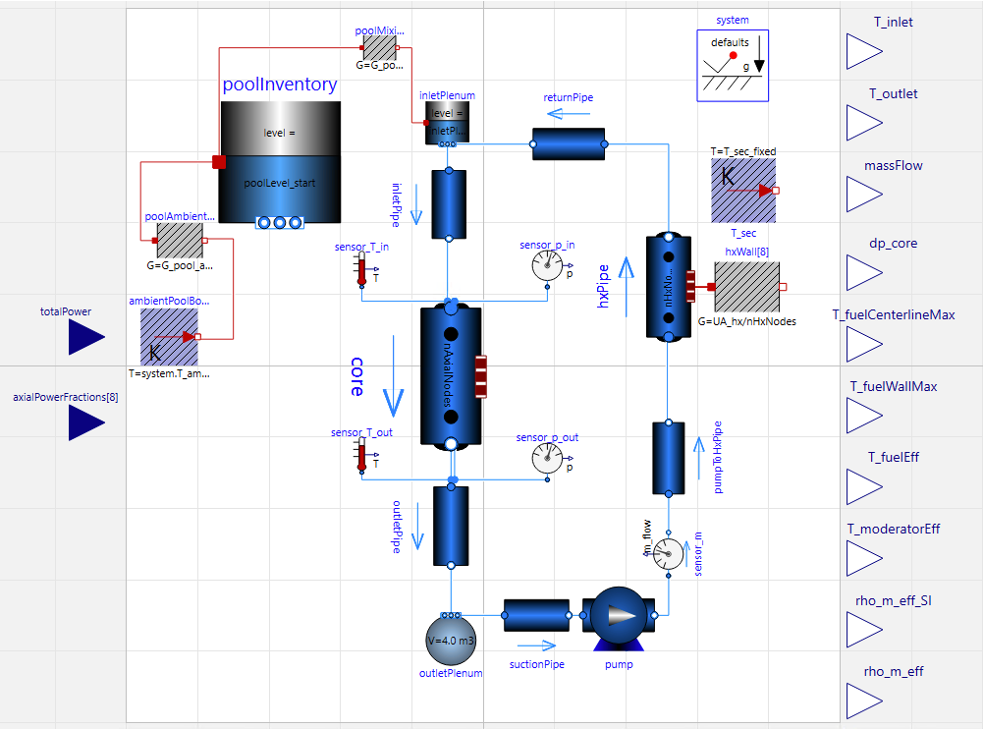
\includegraphics[width=0.76\textwidth]{modelica.png}
  \caption{Modelica thermal-hydraulics model coupled to the Python backend
  through an FMI 2.0 co-simulation FMU.}
\end{figure}

The FMU is advanced at 0.1 s simulated-time intervals using the average power
over each batch.  Thermal feedback is applied only when the returned snapshot
has source \texttt{fmu}; the fallback thermal model can keep the HMI populated
but contributes zero feedback reactivity.

The thermal model is an aggregated system model rather than the OpenMC
geometry itself.  Its current fuel heat structure uses six equivalent rings,
0.5 cm fuel thickness, 7 cm coolant gaps, radii 4.5--50 cm, and a 1.5 m active
height.  The published neutronics reference uses seven resolved fuel rings and
a 3.0 m active height.  This geometry mismatch is a current coupling
limitation: power and effective feedback signals are exchanged, but material
regions are not mapped one-to-one, and the axial heat-source input still comes
from the legacy spatial helper.  The thermal equations and FMU interface are
documented in \path{docs/TH_latex/ThermalHydraulics.pdf} and
\path{docs/fmu_coupling.md}.

\subsection{Current status and verification}

The adapter and export configuration support the listed 1, 2, 4, 8, 16, 25,
40, and 70 group structures.  The documented diffusion benchmark table
currently contains resolved clean-core results through 16 groups; support for a
group structure should not be confused with a completed mesh/runtime
verification at that group count.  The workflow document
\path{docs/diffusion_mgxs_workflow.md} records the current comparison:

\begin{itemize}
  \item OpenMC multigroup transport with the validation-only P0 correction
        approaches the continuous-energy reference as the group structure is
        refined: the reported MG biases are $+806$, $+426$, $+166$, and
        $+66$~pcm for 2, 4, 8, and 16 groups, respectively.
  \item The uncorrected diffusion bias (diffusion $k_{\mathrm{eff}}$ minus
        OpenMC MG $k_{\mathrm{eff}}$) stabilizes around $-400$ to $-500$~pcm
        for the documented 4, 8, and 16 group cases.  This is evidence of a
        repeatable residual bias, not proof that diffusion closure alone is
        its cause.
  \item The resolved two-group diffusion result is anomalous relative to that
        trend: its bias is about $+1194$~pcm relative to two-group OpenMC MG.
        This points to sensitivity to the very broad energy condensation and
        groupwise diffusion coefficients rather than a simple monotonic
        group-count convergence law.
  \item The resolved one-group diffusion result carries an approximately
        $+1800$~pcm bias relative to continuous energy.  Because the fuel rings
        remain spatially resolved in this calculation, that result cannot be
        attributed to collapsing the rings into one spatial region.
\end{itemize}

The clean online result is qualified by the current service because its
$k_{\mathrm{eff}}=1.001429$ is within about 1 pcm of the associated
continuous-energy reference, well inside the 21.75 pcm one-sigma uncertainty.
The clean displayed power shape uses the CE correction described above.  This
qualification is specific to the clean four-group webapp calculation; it is
not an SPH qualification.

The SPH fitting, application, fingerprinting, cache, and qualification
machinery are implemented and unit tested, but the workflow is paused.  Trial
factor sets are archived for later investigation and are not loaded online.
Rodded Core results remain provisional, and discontinuity factors, true
rodded MGXS, and rod-dependent transport corrections remain deferred.

\section{How the modeling layers relate}

\begin{center}
\small
\begin{tabular}{p{3.2cm}p{4.0cm}p{5.3cm}}
\toprule
Layer & Model & Purpose \\
\midrule
OpenMC MGXS export & Resolved-cell multigroup & Generate transport-derived group constants and scattering matrices from continuous-energy Monte Carlo \\
\rule{0pt}{13pt}%
Reference-data loaders & JSON, XML, and CSV adapters & Validate and provide immutable OpenMC-derived runtime inputs \\
Overview page & 0D six-group point kinetics & Evolve reactor amplitude from rod worth and FMU thermal feedback \\
Modelica FMU & Reduced primary-loop and fuel heat structure & Convert power and axial shape into coolant, fuel, and moderator feedback state \\
Core page & Four-group 2D finite-volume diffusion & Solve and display resolved-cell flux and CE-corrected power shape \\
\bottomrule
\end{tabular}
\end{center}

The runtime workflow is:
\begin{enumerate}
  \item publish OpenMC reference artifacts offline;
  \item initialize point kinetics at the CE critical rod position;
  \item advance point kinetics and batch its power into the Modelica FMU;
  \item feed effective FMU temperatures and density back into reactivity;
  \item solve or reuse the four-group diffusion field at the current rod
        position for the Core page;
  \item apply the fixed clean CE power-shape correction to the Core display;
  \item separately derive the FMU axial fractions from the legacy one-group
        shape helper.
\end{enumerate}

\section{Important assumptions and limitations}

The current application remains an educational simulator:
\begin{itemize}
  \item point kinetics assumes one global neutron-population amplitude and six
        lumped precursor groups;
  \item the displayed absolute flux scale is inherited from the legacy
        one-group model;
  \item one effective rod bank stands in for a detailed control system;
  \item rodded diffusion uses equivalent absorption and a fixed clean CE power
        correction rather than rodded MGXS;
  \item the Modelica heat structure is aggregated and does not share a
        one-to-one mesh or geometry with the OpenMC model;
  \item the FMU axial power fractions still come from the legacy one-group
        diffusion helper rather than the four-group CE-corrected map;
  \item fallback thermal values do not contribute reactivity feedback;
  \item no xenon, burnup, fuel depletion, boiling/void feedback, or detailed
        secondary-side control is modeled;
  \item discontinuity factors and runtime SPH are not applied;
  \item time-dependent multigroup solves are not implemented in the web backend.
\end{itemize}

The resolved MGXS remain flux-weighted averages within each OpenMC tally cell,
even though the adapter preserves every exported cell as a separate diffusion
region.  The model is not pin-resolved and is not a licensing-grade core code.

\section{Conclusion}

OpenMC defines the current reactor and publishes the compact data consumed by
the application.  Point kinetics provides fast amplitude dynamics, the
Modelica FMU closes the temperature and density feedback loop, and the
four-group finite-volume solver provides the spatial Core view.  The clean
diffusion result reproduces its associated CE eigenvalue and uses CE data to
correct the displayed power shape.  The rodded spatial treatment and absolute
flux normalization remain the clearest next physics improvements.

The executable interfaces to this model are
\path{backend/openmc_to_diffusion.py},
\path{openmc/diffusion_concentric_reactor.ipynb}, and the two webapp pages.
Detailed operational contracts are kept in
\path{docs/diffusion_mgxs_workflow.md},
\path{docs/fmu_coupling.md}, and
\path{docs/system_architecture.md}.

\end{document}
